% http://www.idsc.ethz.ch/education/theses-semester-projects.html
% IDSC LaTeX Thesis Template
% 
% Author(s):	Eric Müller
% 				Institute for Dynamic Systems and Control
% 				Swiss Federal Institute of Technology (ETH) Zurich
% 
% Created:		2004/04/02  (Eric Mueller)f
% 
% Notes: Has been tested on Windows 7 + MikTeX + TeXnicCenter
%
% Revisions: 	2009/05/29  (Soren Ebbesen)
% 				    2011/03/22	(Soren Ebbesen)
%             2013/03/08	(Soren Ebbesen)
%             2014/03/13	(Soren Ebbesen)
% ______________________________________________________________________________
\documentclass[12pt,twoside,a4paper,fleqn]{report}

%\usepackage[utf8]{inputenc}
\usepackage[english]{ethidsc} % Special IDSC styles and commands      	
								 % {german}/english: language of headings, etc.
								 % {st}/bt/mt: {semester}/bachelor/master thesis\usepackage[francais]{babel} 


 

							
% Page header (don't change)____________________________________________________
\setlength{\parindent}{0em}                 % Disable parindent
\rhead[\nouppercase{\rightmark}]{\thepage}  % Special headings
\lhead[\thepage]{\nouppercase{\leftmark}}   % Special headings
\cfoot{}                                    % Special headings


% Title page (please fill in)___________________________________________________
\title{Projet Ingénierie du Web:\\Application Web pour automatiser la génération des emplois du temps}

\studentA{ABOUNACEUR Younes\\BAIROUF Redone\\BENIMMAR Maryam\\CHAHBI Asmae}
%\==ethidA{97-906-739}
%\==semesterA{5}
%\emailA{muster@student.ethz.ch}


%\studentB{Second Student}
%\ethidB{12-345-678}
%\semesterB{9}
%\emailB{second@student.ethz.ch}

\supervision{Mr EL HAMLAOUI Mahmoud}
\date{2019/2020}



\infopage
\declaration

% Begin document________________________________________________________________
\begin{document}

\maketitle 							% Create title page


% Preamble______________________________________________________________________

\pagenumbering{roman} 				% Begin roman page numbering (i,ii,...)

\chapter*{Remerciements}
\addcontentsline{toc}{chapter}{Remerciements}

C’est avec un grand plaisir que nous réservons ces quelques lignes en signe de gratitude et de profonde reconnaissance à tous ceux qui, de près ou de loin, ont contribué à la réalisation et l’aboutissement de ce travail.  \\
  
Tout d’abord  nous remercions notre encadrant \emph{Mr EL HAMLAOUI Mahmoud} pour son soutient, sa disponibilité, ses précieux conseils et son aide tout au long de l’élaboration de ce travail. \\

Nous nous acquittons, enfin, volontiers d’un devoir de gratitude et de remerciements à tous les professeurs qui nous ont enseigné pendant ces deux dernières années, pour le
savoir qui nous ont transmis et pour leur entière disponibilité.
\newpage

\chapter*{Résumé}

\addcontentsline{toc}{chapter}{Résumé}
\noindent \textbf{FlOp EDT} est une application web qui permet de générer d'une manière automatique un emplois du temps au sein d'une école universitaire. d'une façon qui satisfait les contraintes de tous les professeurs intervenants, ce qui facilite le long processus de communication qui se repète presque à chaque semaine entre le responsable de fillière et les professeurs donnant des cours pendant la semaine.\\

Ce document a pour but de décrire le déroulement de notre projet Ingénierie du web.\\

Nous vous présenterons donc tout au long du rapport, les étapes de la réalisation de ce projet, ainsi que les outils que nous avons utilisé pour réaliser notre projet.\\

Au premier lieu, nous allons présenter le contexte général du projet, ensuite nous attaquerons la conception et l'idée générale de l'application, et vers la fin de ce document nous aborderons le coté technique de notre application, en inclurant les outils et les technologies que nous avons appris et utilisé.
\newpage




%{\large\textbf{Mots clés :}}
 %Android , Slim, Bootstrap, MySQL

\chapter*{Abstract}
\addcontentsline{toc}{chapter}{Abstract}

\textbf{FlOp EDT} is a web application that automatically generates a timetable within a university school. in a way that satisfies the constraints of all the participating teachers, which facilitates the long process of communication which is repeated almost every week between the tutor and the teachers giving lessons during the week. \\

The purpose of this document is to describe the progress of our Web engineering project. \\

We will therefore present throughout the report, the stages of the realization of this project, as well as the tools that we used to carry out our project. \\

First, we will present the general context of the project, then we will attack the design and the general idea of the application, and towards the end of this document we will discuss the technical side of our application, including the tools and technologies that we have learned and used.
\newpage


\listoffigures
\tableofcontents
\clearpage 

% Chapters______________________________________________________________________

\pagestyle{fancy}               	% Fancy headings
\pagenumbering{arabic}				% Begin arabic page numbering (1,2,...)

\pagenumbering{arabic}
\chapter*{Introduction}
\addcontentsline{toc}{chapter}{Introduction Générale}
Afin d’appliquer les méthodologies et les notions enseignées durant le cours d'Ingénierie du Web, nous sommes invités à réaliser un projet qui nous permet d’appliquer nos connaissances théoriques sur le champ pratique.\\

Dans toute établissement universitaire, bien organiser l'emplois du temps est l'une des tâches les plus prioritaires du directeur ou du responsable de fillière.

Notre projet se situe dans ce contexte, il s’agit d’une application web qui automatise le processus de génération de l'emplois du temps, ce qui va faciliter la vie pour le responsable de fillière.\\

Le présent rapport est dédié à la présentation de l'ensemble des travaux menés dans le cadre de notre projet. Le premier chapitre est destiné à la description du contexte général de ce projet, allant de l'amenant, la problématique, aux objectifs du projet.\\

Le deuxième chapitre aborde dans un premier temps une étude et une analyse des besoins, en commençant par l'étude de l'existant, ensuite l'analyse des fonctionnalités à implémenter. Puis, en proposant en deuxième lieu une conception technique de l'application.\\

Le dernier chapitre est destiné à décrire la mise en oeuvre du projet, il contient les outils choisis pour le développement ainsi que les détails des différentes phases de réalisation de l'application.\\

Enfin, la conclusion générale résume le bilan du travail effectué et les principales perspectives.\\
\newpage














%Ce rapport peut ainsi être subdivisé en cinq parties :
%\begin{itemize}
%\item kmkkkm
% \end{itemize}
% 



\chapter{Contexte général du projet}
Dans ce chapitre nous allons définir le contexte général du projet et ses objectifs
\newpage

\section{Amenant}
L'ingénierie du web, est l'une des spécialités les plus demandées dans le monde du travail, et autant que étudiants 2éme année Géniel logiciel à l'ENSIAS, c'est une capacité qu'on doit maitriser, du coup, nous sommes menés à réaliser une application web en se  basant sur ce qu'on a vu dans le cours d'ingénierie web avec Mr EL Hamlaoui.\\


\section{Problématique}
Au sein de toute université dans le monde, les étudiants et les professeurs doivent respecter un emplois du temps. Or, la création de cet emplois du temps prend beacoup du temps et d'effort par la personne en charge, généralement c'est le chef de fillière. Ce dernier doit contacter chaque professeur et voir quand est ce qu'il est disponible, par la suite il doit créer un emplois qui respecte au maximum possible les contraintes du disponibilité des profs, et finalement il contacte les profs pour vérifier si l'emplois proposé est convenable pour eux.\\


\section{Analyse de besoin}
Afin de faciliter cette tâche pour le chef de fillière, et automatiser ce long processus qui inclut plusieurs intervenants, nous avons adapté et amélioré une application web \textbf{FlOp EDT} qui génére un emplois du temps qui satisfait les professeurs et qui est validé par le chef de fillière.\\

\section{Objectifs du projet}
Parmis les tâches pour réaliser un bon déroulement du projet:\\
\begin{itemize}
\item Adapter la base de données, pour qu'elle contienne les noms des profs, les salles et les modules de l'ENSIAS.
\item Améliorer le design et l'interface de l'application.
\item Améliorer la performance de l'application et fixer quelques problèmes fonctionnelles.
\item Visualisation des résultats.
\end{itemize}


\clearpage
\clearpage
\chapter{Analyse et conception}
Ce chapitre présente l'étude de l'existant avec une analyse et description des besoins, ainsi que les étapes établies pour réaliser le projet.
\newpage

\section{Étude et analyse des besoins}
\subsection{Étude de l'existant}
La gestion de l'emplois  du temps est une tâche trés importante que ça soit pour les étudiants ou bien les professeurs, plusieurs parmis les étudiants içi à l'ENSIAS trouvent que parfois l'emplois du temps n'est pas publié tôt, mais le fait de contacter chaque professeur et arriver à un compromis qui satisfait tout le monde, prend énormement du temps de chef de fillère. D'où vient le besoin à une application web qui automatise ce long processus.
\subsection{Capture des besoins}
Le projet qui nous a été accordé consiste à répondre aux besoins suivants:
\subsubsection{Besoins fonctionnels}
\begin{itemize}
    \item La possibilité pour les profs de choisir les heures pendant les quelles ils seront disponibles.
    \item Gestion des utilisateurs.
    \item Génération un emplois du temps en se basant sur la disponibilté des professeurs et des salles.
    \item Génération un fichier qui peut être téléchargé est inséré dans Google Calendar pour rappeller un prof qu'il a un cours ou un TD à une heure donnée.
\end{itemize}

\subsubsection{Besoins non-fonctionnels}
\begin{itemize}
  \item maintenabilité: L'application doit être facile à maintenir, de manière cohérente et à moindre coût, en état de fonctionnement, pour laisser la possibilité à d'autres ingénieurs de modifier l'appication et l'adapter selon le besoin d'une autre école.
  \item  Efficacité: L'application doit marcher correctement sans erreurs.
  \item  Simplicité : L'interface doit être simple et facile à utiliser.
  \item Sécurité : L'application contient des données de l'école, et donc il faut les protéger en procédant par des logins et mots de passe.
  \item Disponibilté : L'application doit être tout le temps à la disposition de l'utilisateur.
   
\end{itemize}  

\section{Conception de la solution}

\subsection{Diagramme de classes}
 \begin{figure}[!htb]
      \centering
        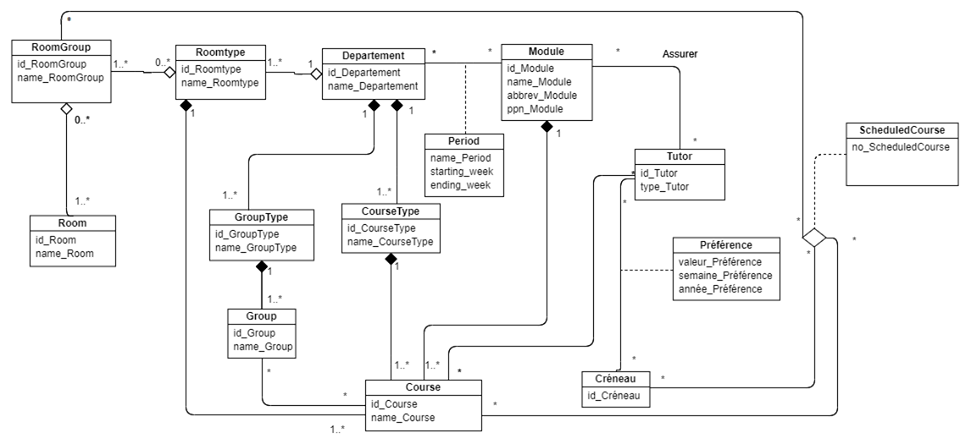
\includegraphics[width=17cm,height=21cm]{img/ClassDiagramm.png}
        \caption{Scénario :Diagramme de classe. }
    \end{figure}
\newpage

\\
\subsection{Diagramme de cas d'utilisation}
 \begin{figure}[!htb]
      \centering
        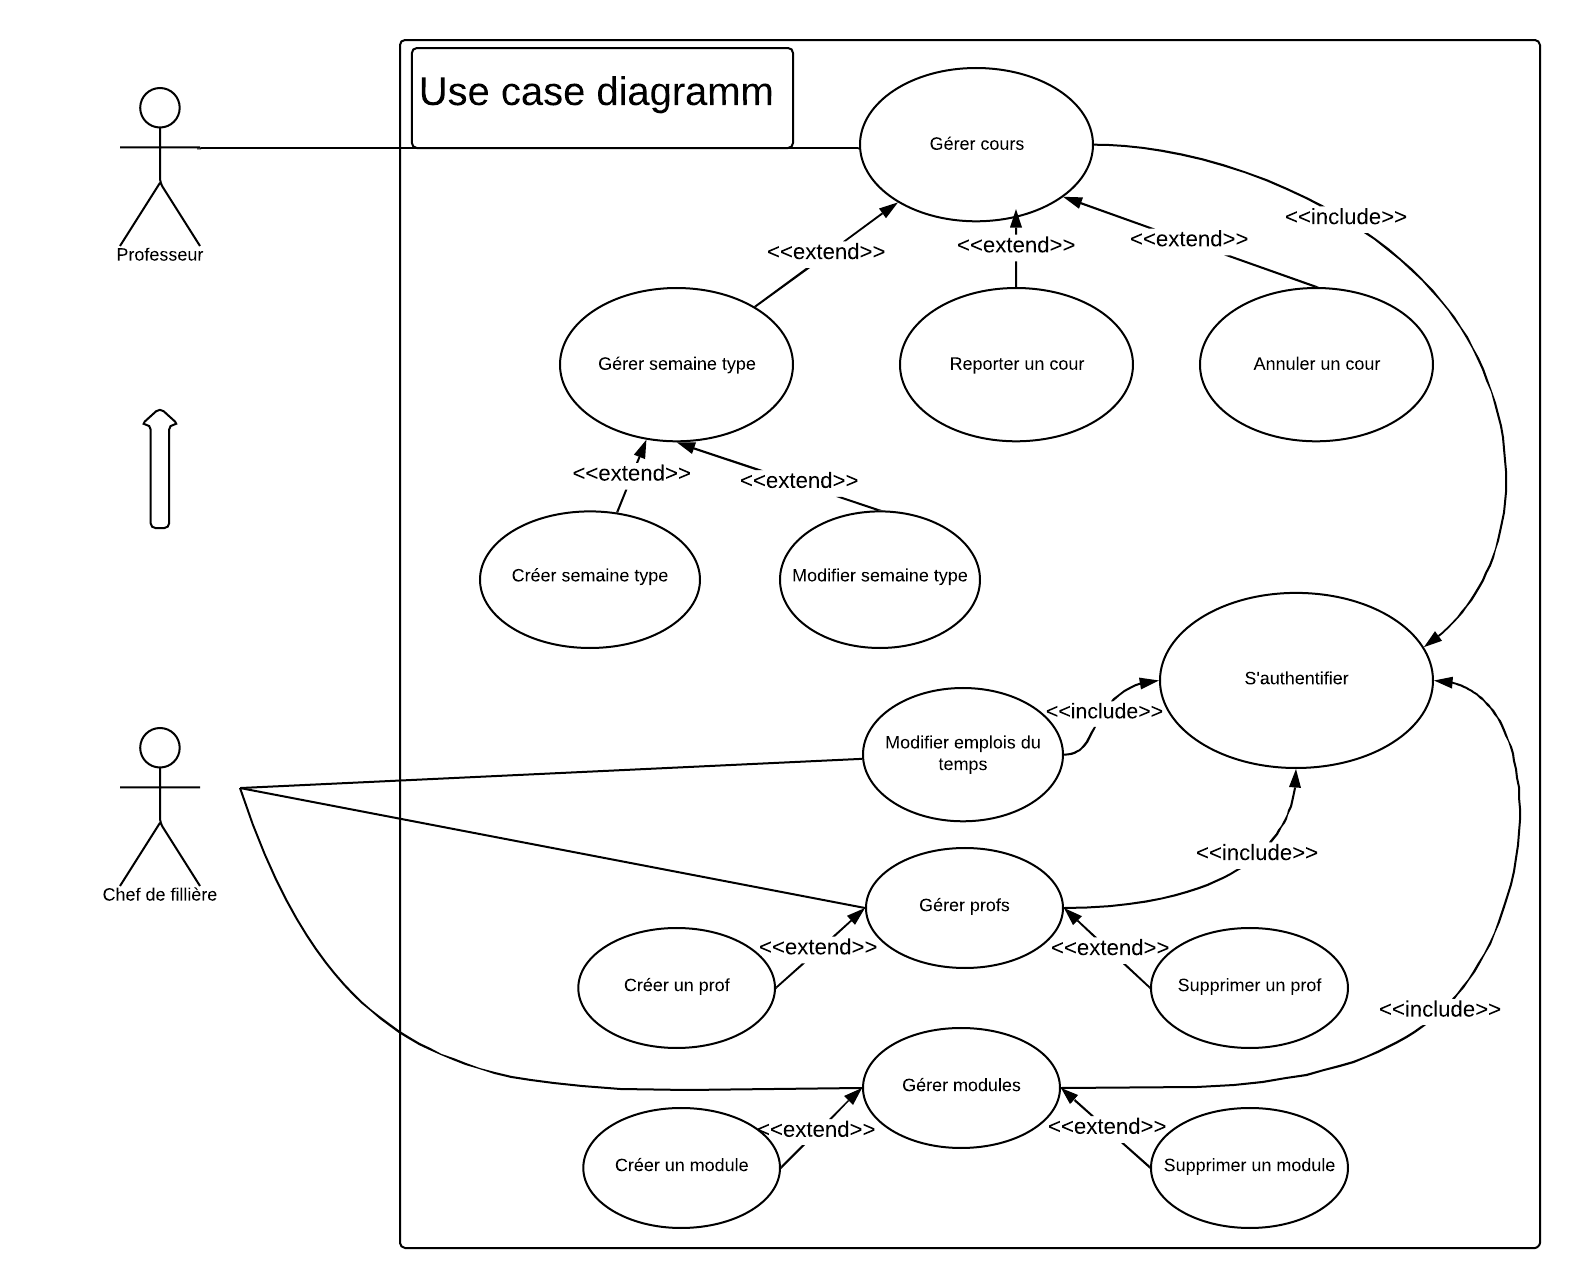
\includegraphics[width=15cm,height=18cm]{img/UseCase.png}
        \caption{Diagramme de cas d'utilisation. }
    \end{figure}
\newpage 

\subsection{Diagrammes de séquence}
Les diagrammes suivants représentent quelque scénarios possibles pour l'utilisateur de l'application que ça soit le prof ou le chef de fillière:
\subsubsection*{S'authentifier}
L'utilisateur saisi sont login et mot de passe, en cas d'erreur l'application lui demande de retaper les informations demandées.
 \begin{figure}[!htb]
      \centering
        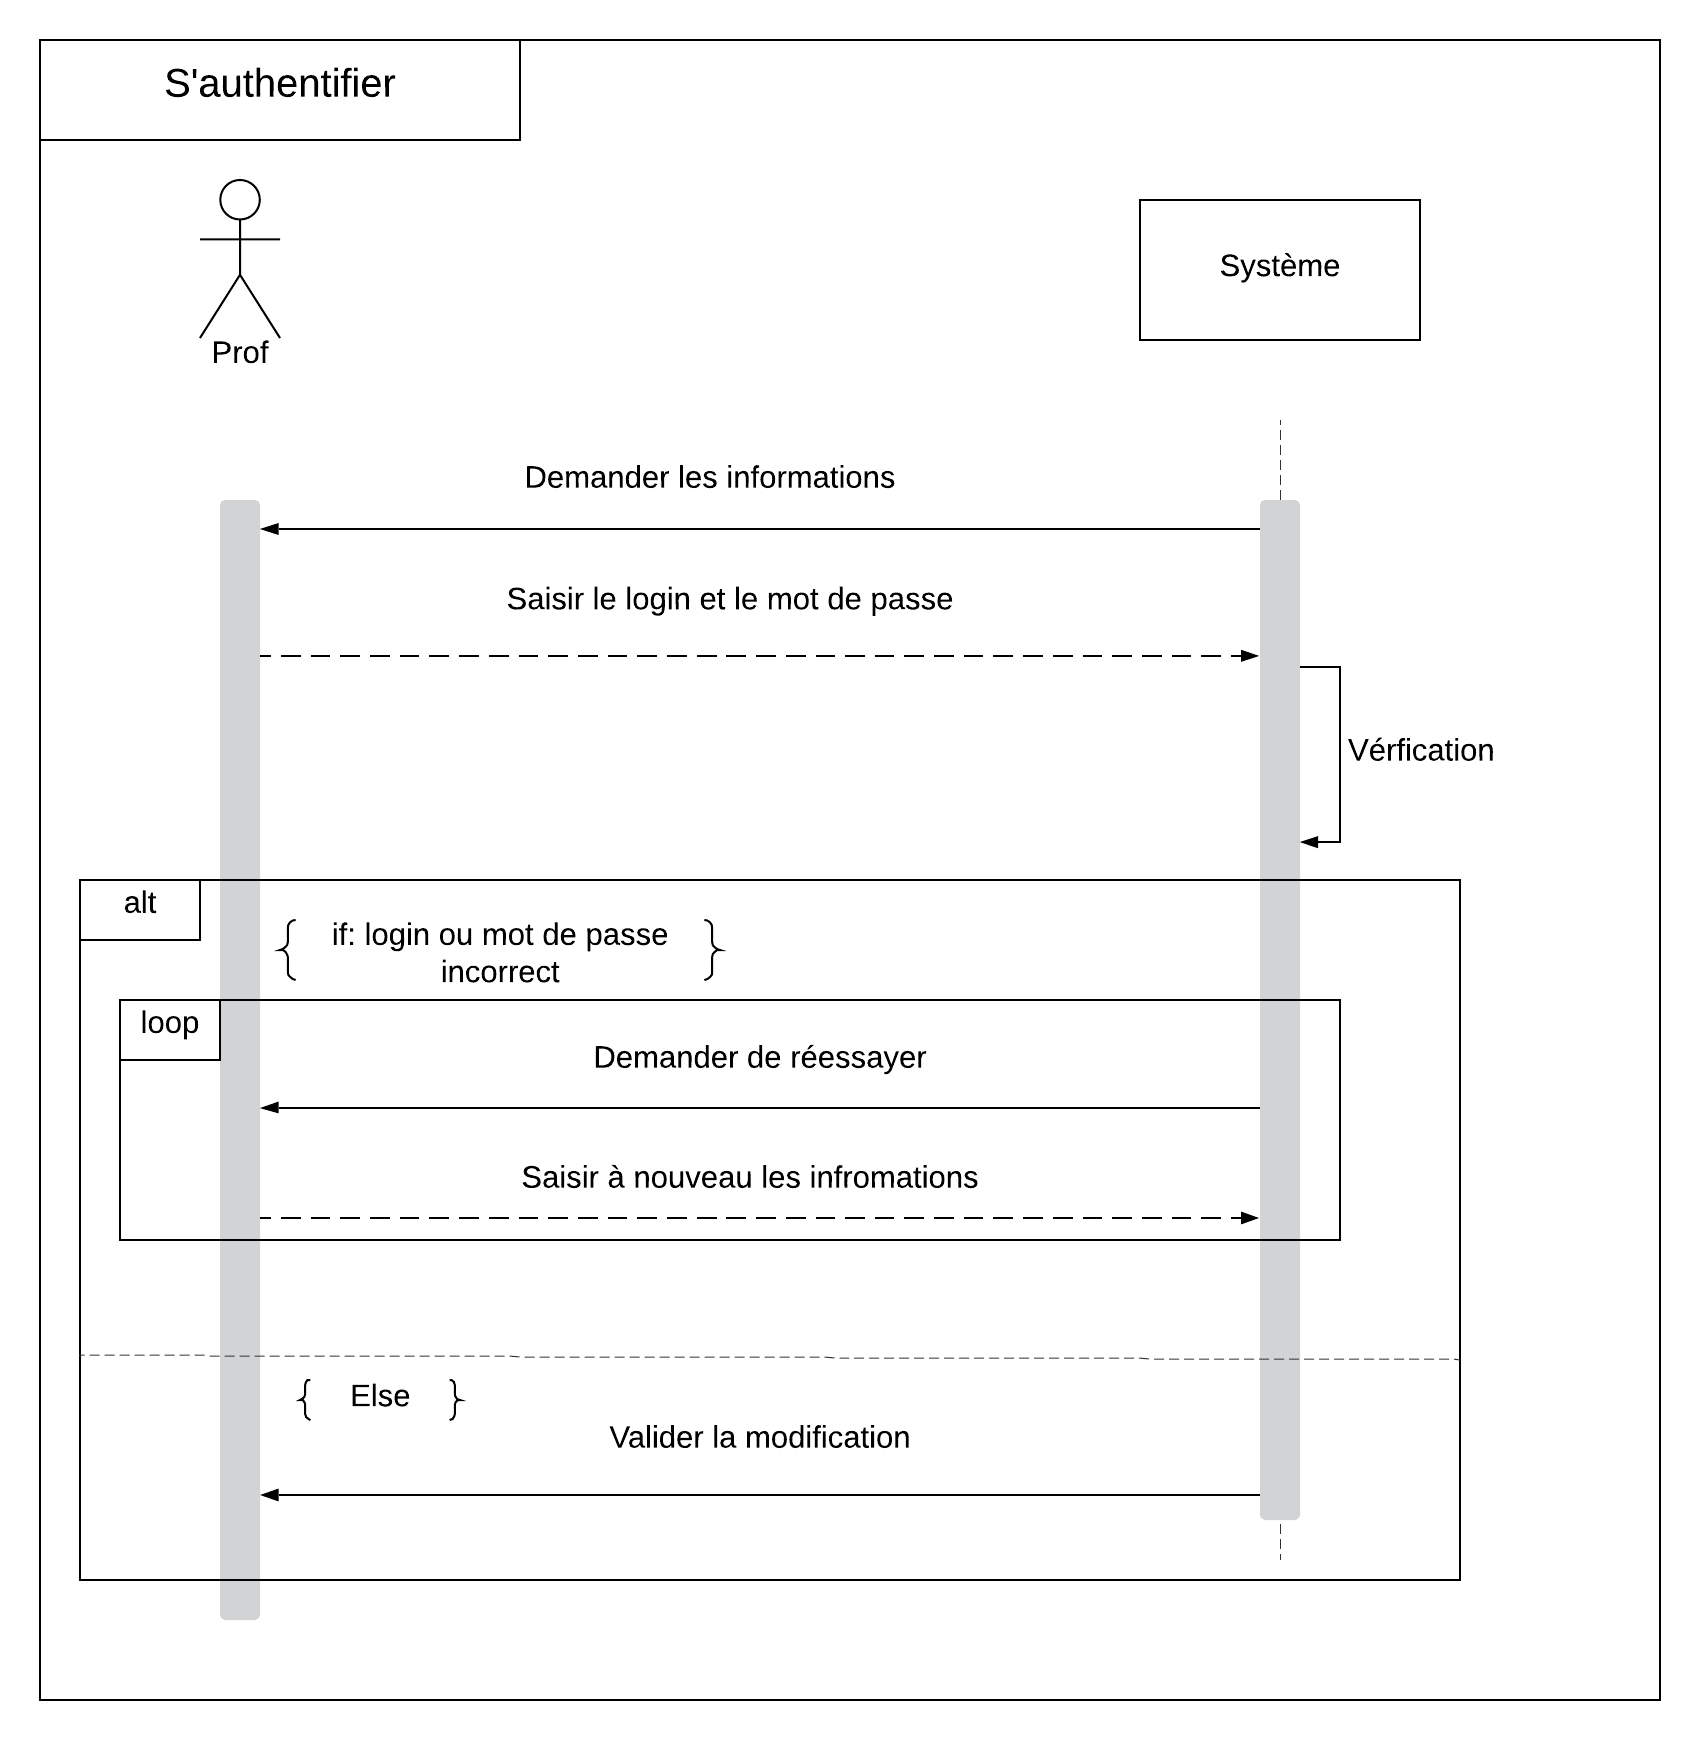
\includegraphics[width=15cm,height=16cm]{img/S'authentifier.png}
        \caption{Scénario d'authentification. }
    \end{figure}
    
\newpage

\subsubsection*{Créer semaine type}
Le prof sélectionne les heures pendant les quelles il est disponible.
 \begin{figure}[!htb]
      \centering
        \includegraphics[width=15cm,height=18cm]{img/CréerSemType.png}
        \caption{Scénario :Créer Semaine Type. }
    \end{figure}
\newpage
\subsubsection*{Modifier semaine type}
Le prof modifie les heures pendant les quelles il est disponible, en changeant ses préférences.
 \begin{figure}[!htb]
      \centering
        \includegraphics[width=15cm,height=18cm]{img/CréerSemType.png}
        \caption{Scénario :Modifier Semaine Type. }
    \end{figure}
 \newpage
 \subsubsection*{Reporter un cours}
Le prof peut reporter un cours, en précisant la date du rattrappage, mais s'il y a une contraine qui empêche d'avoir cette nouvelle séance, un message d'erreur est affiché.
 \begin{figure}[!htb]
      \centering
        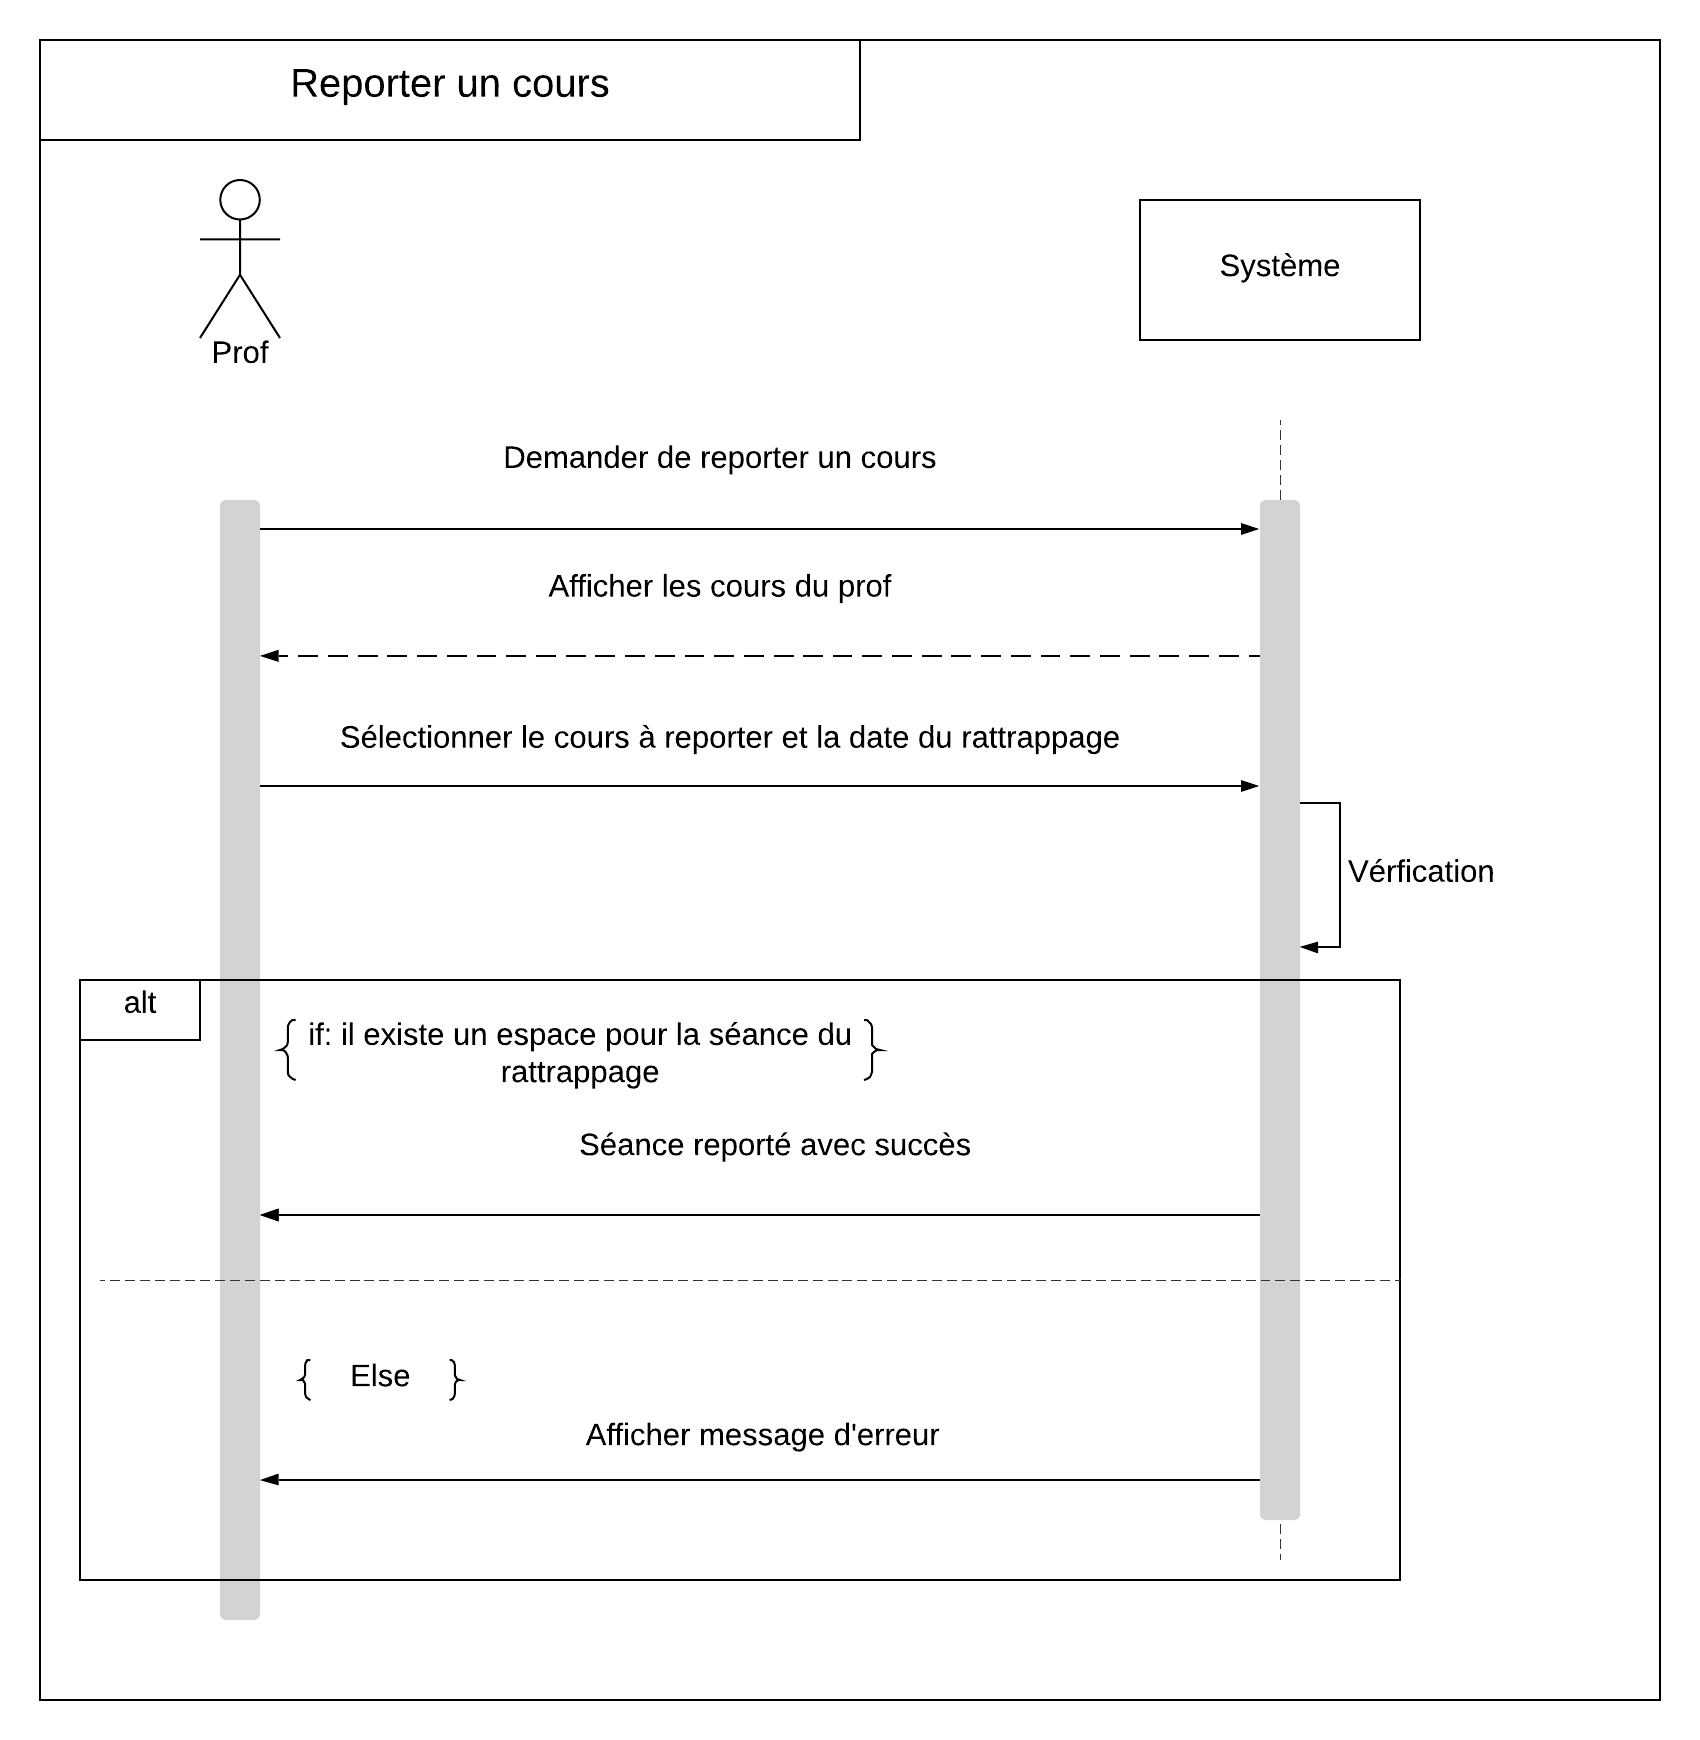
\includegraphics[width=15cm,height=18cm]{img/ReporterCours.png}
        \caption{Scénario :Reporter un cours. }
    \end{figure}   
\newpage
\subsubsection*{Annuler un cours}
Le prof peu annuler un cours.
 \begin{figure}[!htb]
      \centering
        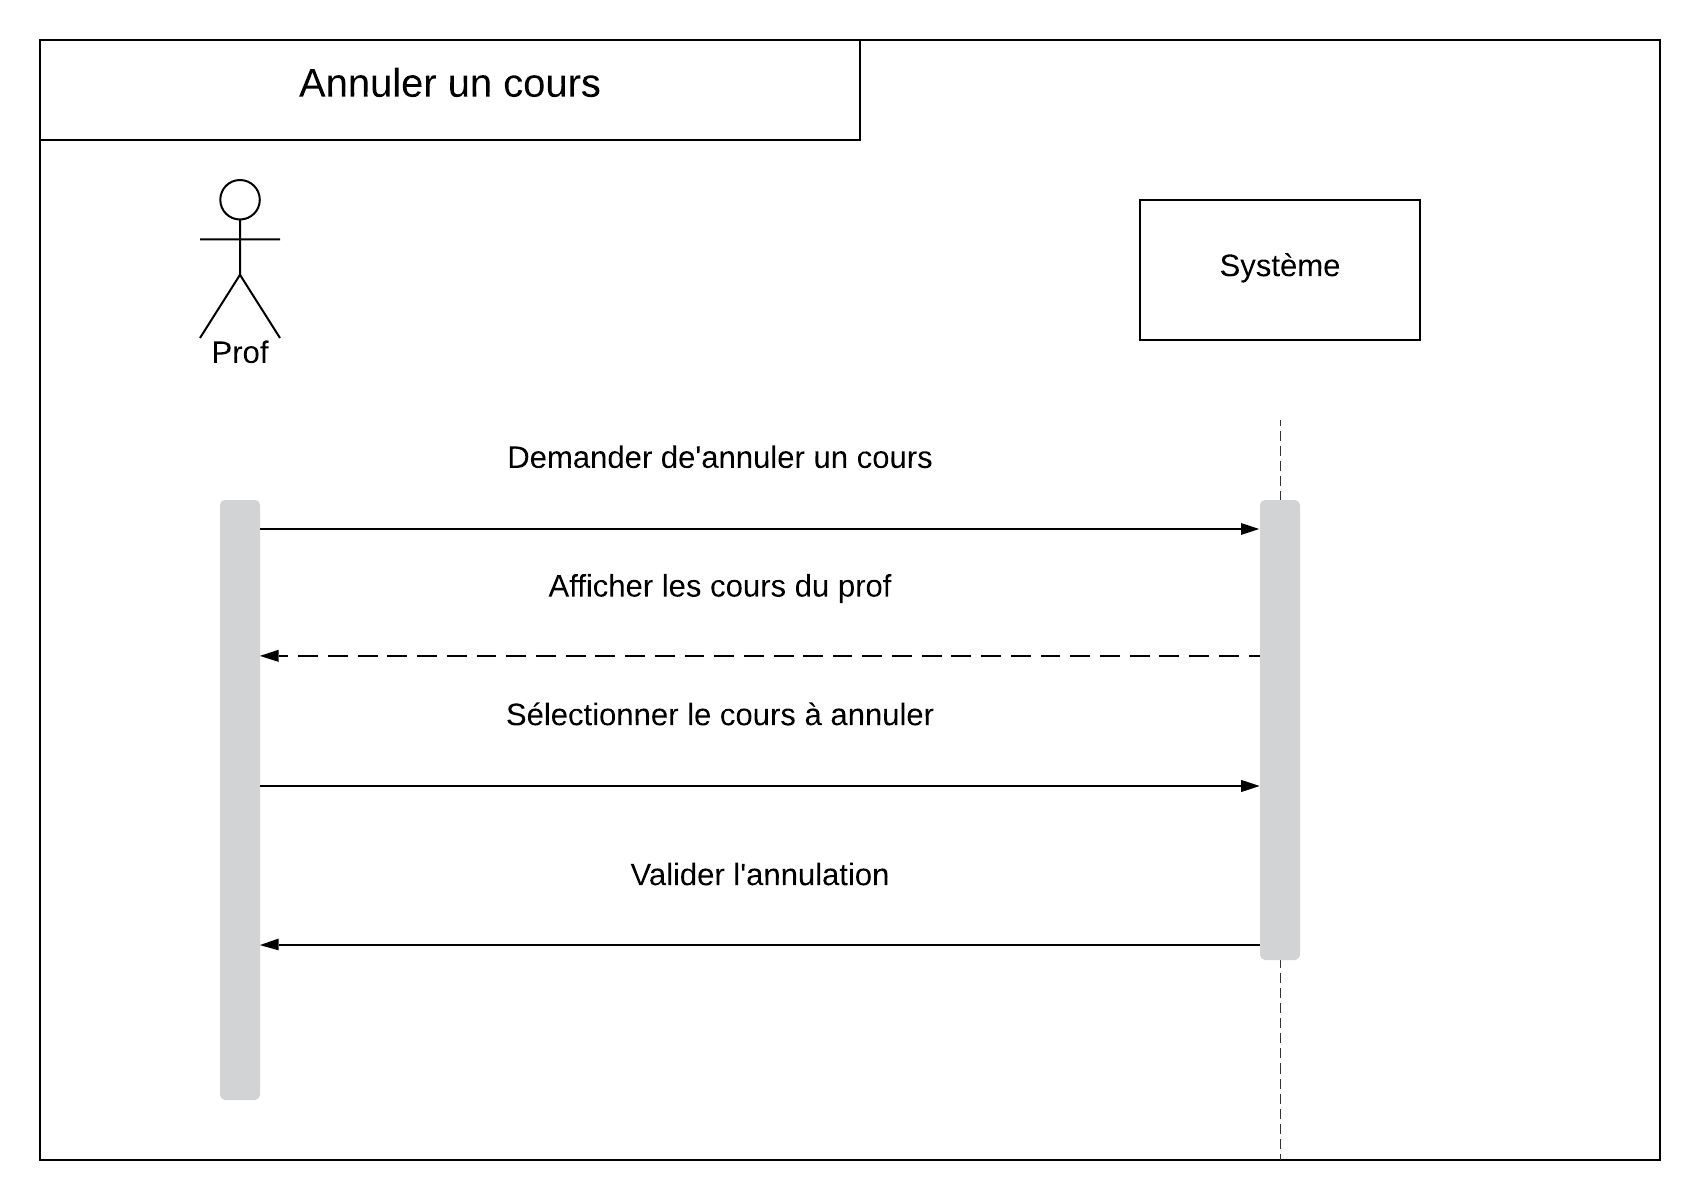
\includegraphics[width=15cm,height=18cm]{img/AnnulerCours.png}
        \caption{Scénario :Annuler un cours. }
    \end{figure}
\newpage
\subsubsection*{Créer prof}
Dans l'interface admin, le chef de fillière peut ajouter un nouveau prof, si un champ est vide, un message d'erreur est affiché.
 \begin{figure}[!htb]
      \centering
        \includegraphics[width=15cm,height=18cm]{img/CréerProf.png}
        \caption{Scénario :Créer un prof. }
    \end{figure}
\newpage
\subsubsection*{Summprimer un  prof}
Dans l'interface admin, le chef de fillière peut supprimer un prof.
 \begin{figure}[!htb]
      \centering
        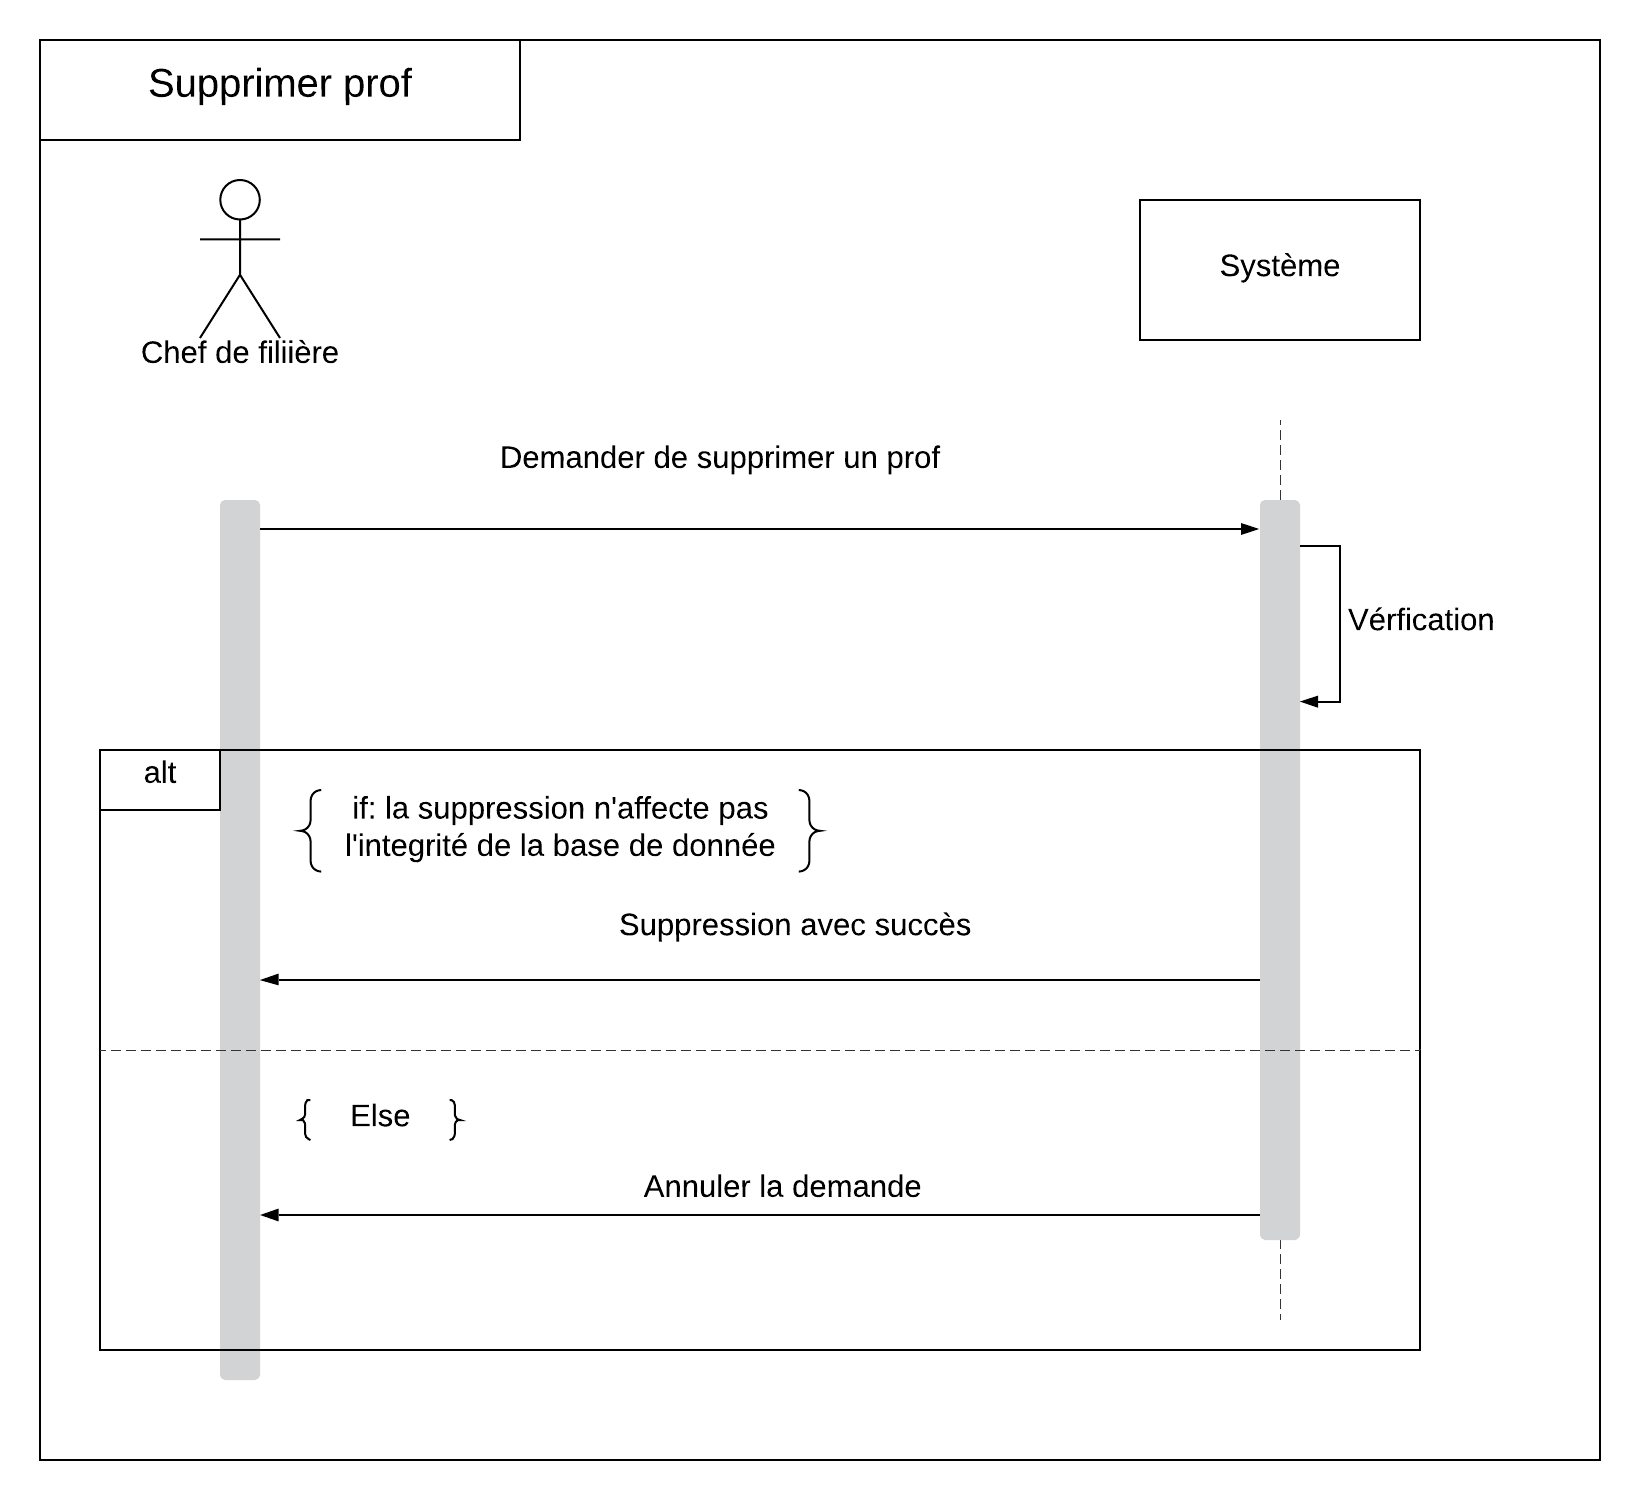
\includegraphics[width=15cm,height=18cm]{img/SupprimerProf.png}
        \caption{Scénario :Supprimer un prof. }
    \end{figure}
\newpage
\subsubsection*{Créer module}
Dans l'interface admin, le chef de fillière peut ajouter un nouveau module, si un champ est vide, un message d'erreur est affiché.
 \begin{figure}[!htb]
      \centering
        \includegraphics[width=15cm,height=18cm]{img/CréerModule.png}
        \caption{Scénario :Créer un module. }
    \end{figure}
\newpage
\subsubsection*{Summprimer un  module}
Dans l'interface admin, le chef de fillière peut supprimer un module.
 \begin{figure}[!htb]
      \centering
        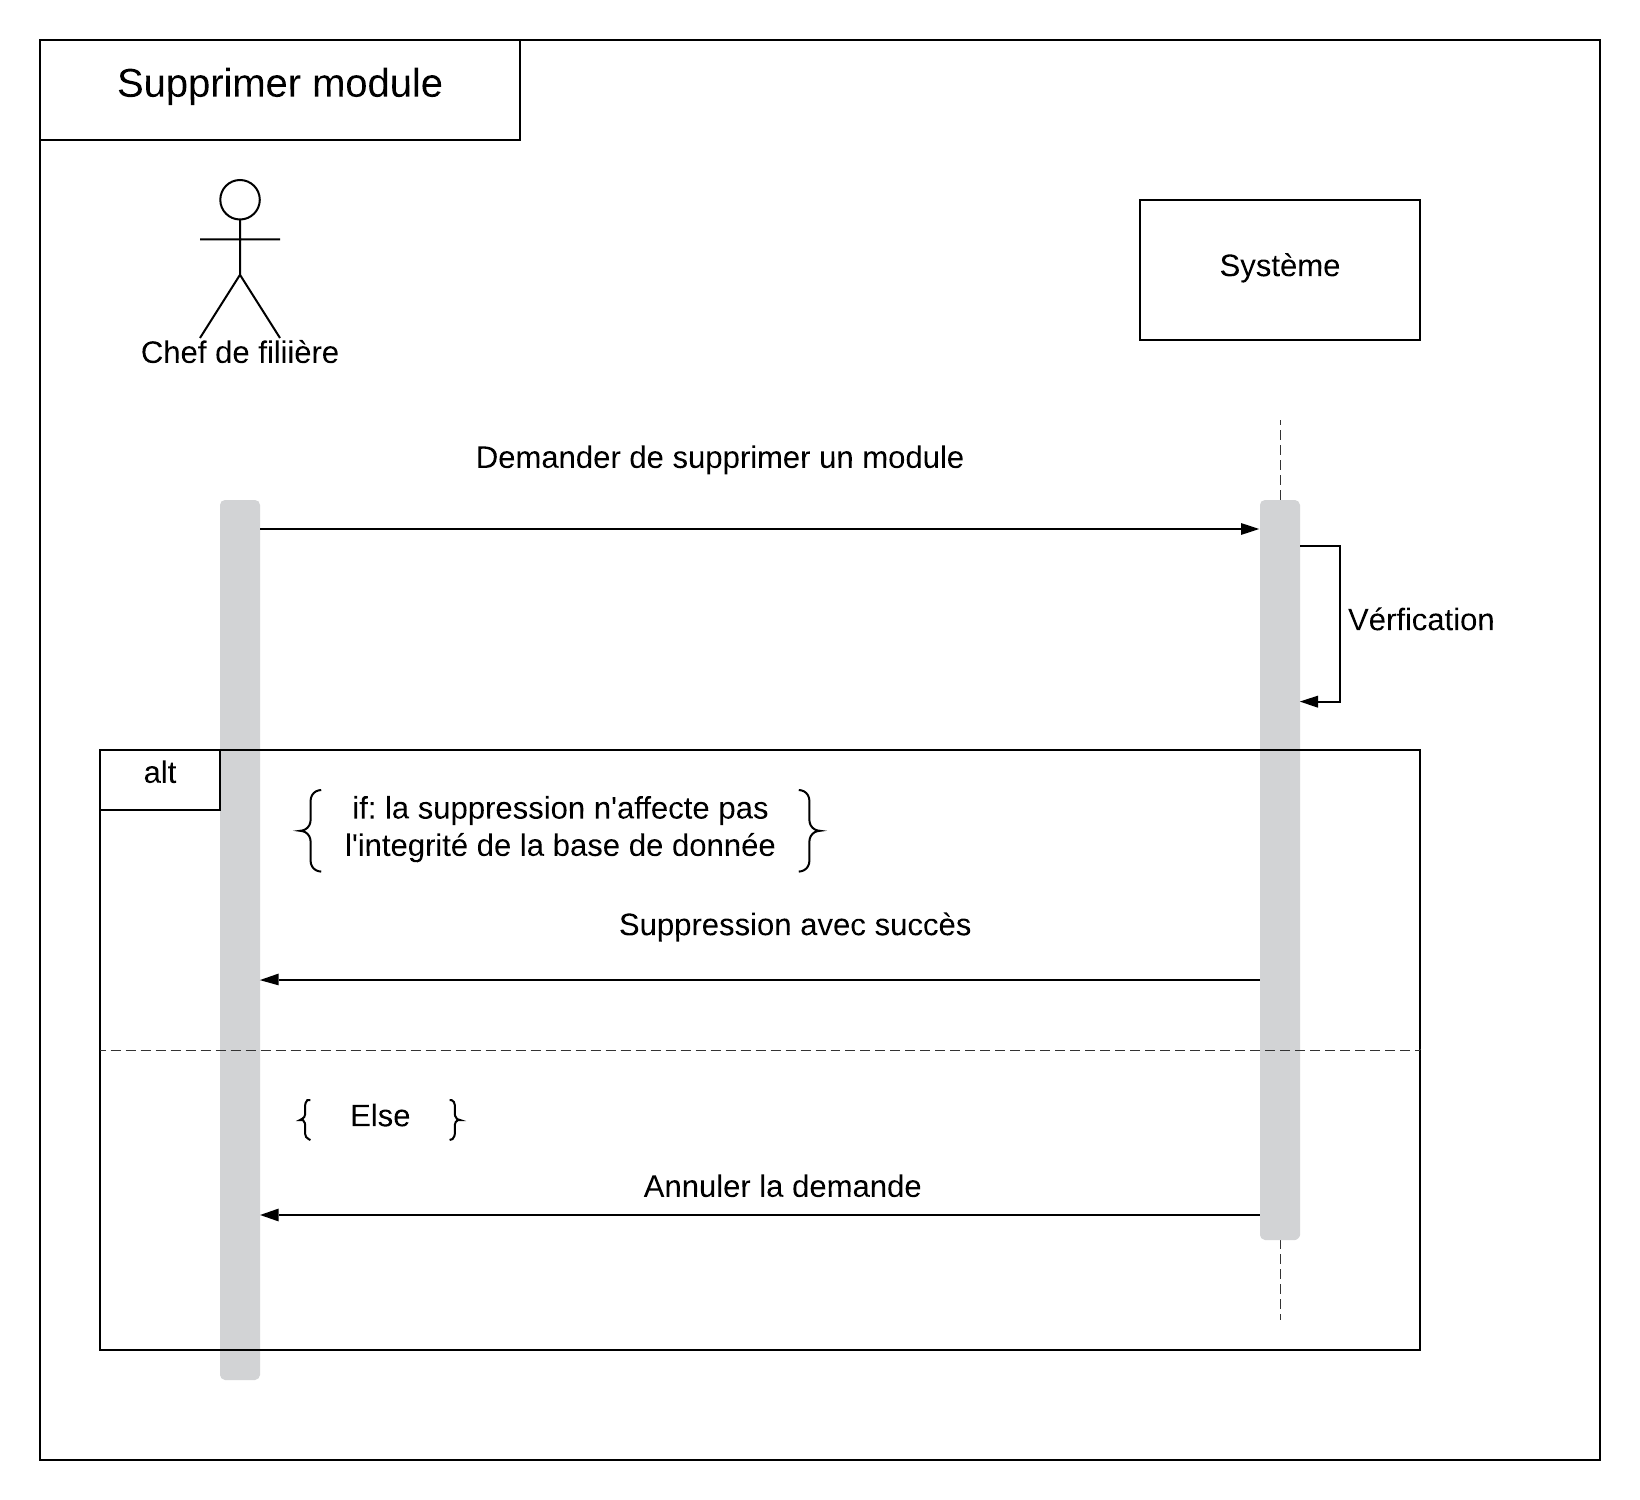
\includegraphics[width=15cm,height=18cm]{img/SupprimerModule.png}
        \caption{Scénario :Supprimer un module.}
    \end{figure}










\clearpage
\chapter{Réalisation et mise en oeuvre}
Ce chapitre aborde la mise en oeuvre et la réalisation, en présentant les outils de réalisation ainsi que le travail réalisé.
\newpage
\section{Outils de développement}
\subsection{Langages de programmation et développement}
\subsubsection*{Python}
Python est un langage de programmation objet, multi-paradigme et multiplate-forme.
Il favorise la programmation impérative structurée, fonctionnelle et orientée objet.
C'est un outil essentiel pour notre projet puisque nous avons utilisé Django.\\

\begin{figure}[h]
      \centering
        
\includegraphics[width=7cm,height=5cm]{img/python.jpg}
        \caption{Logo de Python}
\end{figure}
\subsubsection*{JavaScript}
JavaScript est un langage de  programmation qui nous permet d'implémenter des éléments complexes sur des pages Web. Chaque fois, une page Web ne se contente pas de rester là et affiche des informations statiques que nous pouvons consulter: affichage de mises à jour de contenu actualisées, de cartes interactives, de graphiques 2D et animés. Graphiques 3D, défilement de jukebox vidéo, etc.\\
Nous avons utilisé Java Script pour l'animation de quelque bouttons, et la coloration dynamique de quelques interfaces graphiques dans l'application.
\begin{figure}[h]
      \centering
        
\includegraphics[width=7cm,height=5cm]{img/javascript.png}
        \caption{Logo de JavaScript}
\end{figure}

\subsubsection*{HTML/CSS}
HTML, HyperText Markup Language, donne la structure et la signification du contenu en définissant ce contenu comme, par exemple, des en-têtes, des paragraphes ou des images.\\
CSS, or Cascading Style Sheets, est un langage de présentation créé pour styliser l'apparence du contenu, à l'aide, par exemple, de polices ou de couleurs.\\
\begin{figure}[h]
      \centering
        
\includegraphics[width=7cm,height=5cm]{img/HTMLCSS.png}
        \caption{Logo de HTML et CSS}
\end{figure}

\newline
\subsection{Environement de développement}
\subsubsection*{Django}
Django est un framework Web Python de haut niveau qui encourage un développement rapide et une conception propre et pragmatique. Conçu par des développeurs expérimentés, il prend en charge une grande partie des tracas du développement Web, il nous a permet  donc de nous concentrer sur l'écriture de notre application sans avoir à réinventer la roue. C'est gratuit, open source, sécurisé et rapide.\\
C'est l'outil le plus important pour la réalisation de ce projet, les développeurs originaux l'ont choisi pour sa bonne performance, et donc nous avons choisi de garder le même outil pour faciliter la tâche.
\begin{figure}[H]
      \centering
        
\includegraphics[width=7cm,height=4cm]{img/django-logo.jpg}
        \caption{Logo de Django}
\end{figure}
\newline

\subsubsection*{Visual Studio Code}
Visual Studio Code est un éditeur de code extensible développé par Microsoft pour Windows, Linux et macOS. Il est  open source et gratuit, supportant plusieurs langages.
\begin{figure}[H]
      \centering
        
\includegraphics[width=7cm,height=6cm]{img/VS.png}
        \caption{Logo de Visual Studio Code}
\end{figure}
\newline
\subsubsection{Docker}
Docker est un ensemble de produits en tant que service de plate-forme qui utilisent la virtualisation au niveau du système d'exploitation pour fournir des logiciels dans des packages appelés conteneurs. Les conteneurs sont isolés les uns des autres et regroupent leurs propres logiciels, bibliothèques et fichiers de configuration; ils peuvent communiquer entre eux par des canaux bien définis.
\begin{figure}[H]
      \centering
        
\includegraphics[width=7cm,height=6cm]{img/Docker_logo.jpeg}
        \caption{Logo de Docker}
\end{figure}

\\
\\
\\
\subsubsection*{PostgreSQL}
PostgreSQL, également connu sous le nom de Postgres, est un système de gestion de base de données relationnelle gratuit et open source qui met l'accent sur l'extensibilité et la conformité aux normes techniques. Il est conçu pour gérer une gamme de charges de travail, des machines uniques au Data Warehouse ou aux services Web avec de nombreux utilisateurs simultanés.\\
Il est utilisé dans ce projet pour la gestion des bases de données.
\begin{figure}[H]
      \centering
        
\includegraphics[width=7cm,height=4cm]{img/PostgreSQL.png}
        \caption{Logo de PostgreSQL}
\end{figure}

\newpage
\section{Réalisation}
\subsection*{S'authentifier:}
Chaque utilisateur a un username qui est simplement l'abréviation de son nom, et le mot de passe : "passe" qui peut être changer par la suite dans la section aide \\
 Pour le chef de fillière il peut entrer avec le username "root". les interfaces affichées et leurs  droits d'accès dépendent évidement de la classe de l'utilisateur. 
\begin{figure}[H]
      \centering
        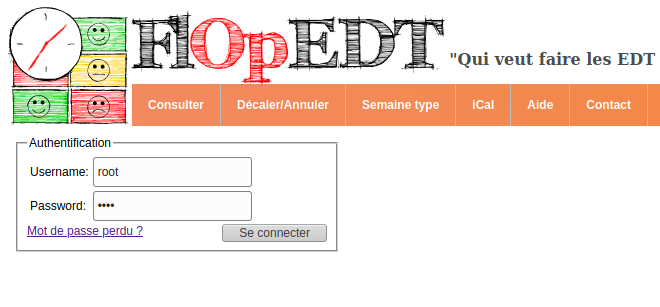
\includegraphics[width=14cm,height=12cm]{img/1.png}
        \caption{Interface login}
\end{figure}
\newpage
\subsection*{Semaine type:}
Si l'utilisateur est un prof, il peut accèder à l'interface "semaine type", pour séléctionner ses préférences, en d'autres termes les heures de son disponibilé et les heures de son non-disponibilité. \\
Il peut également chosir une autre semaine type pour une période spécifique.
\begin{figure}[H]
      \centering
        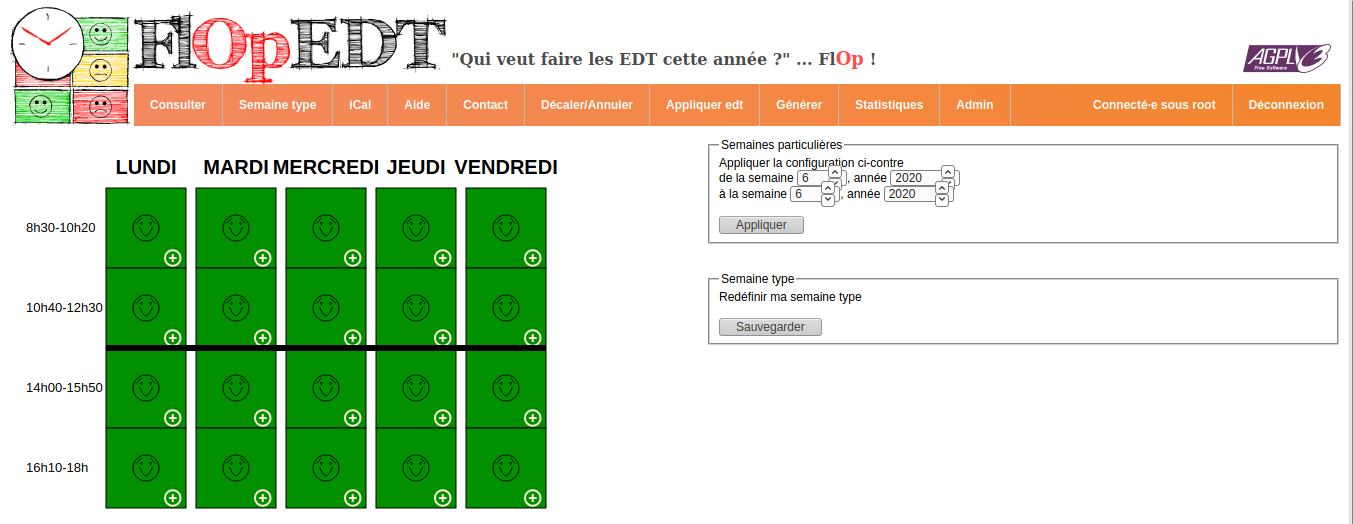
\includegraphics[width=14cm,height=12cm]{img/2.png}
        \caption{Interface Semaine type}
\end{figure}
\newpage
\subsection*{Emploi non encore génére}
Lorsque l'emploi est vide, cette interface va être affichée.
\begin{figure}[H]
      \centering
        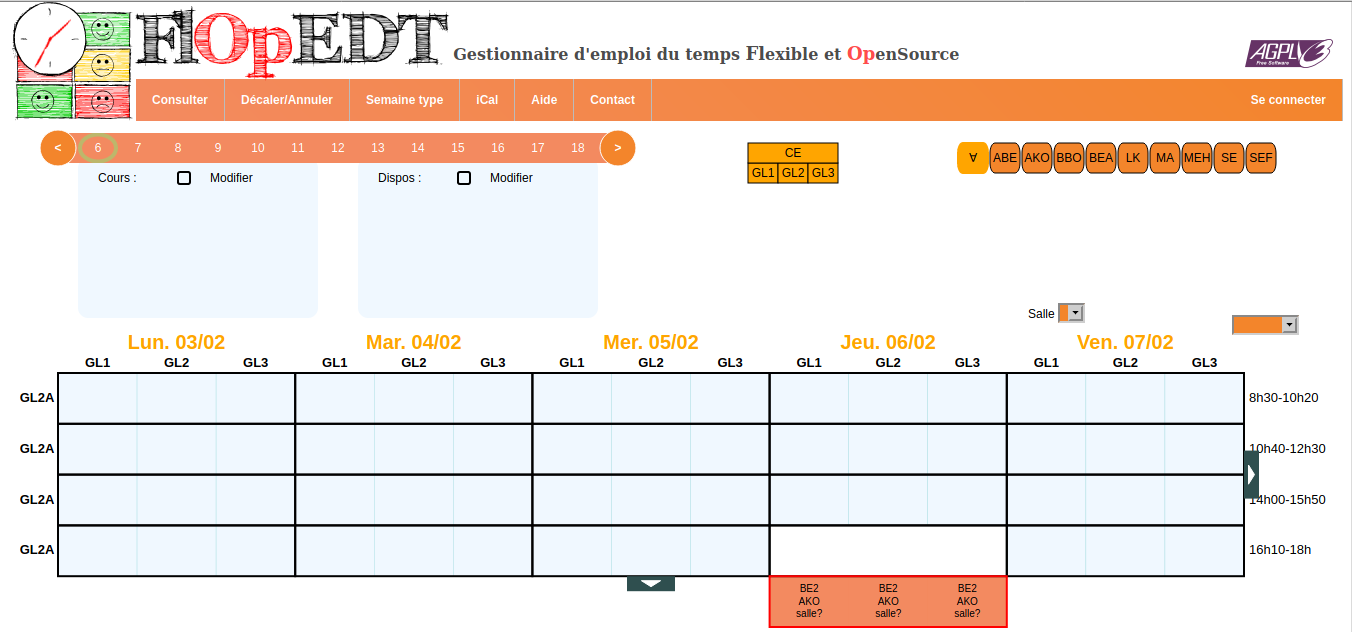
\includegraphics[width=15cm,height=12cm]{img/3.png}
        \caption{Interface Emploi non encore génére}
\end{figure}
\newpage
\subsection*{Générer un Emploi:}
Le chef de fillière a le droit de générer l'emploi du temps via cette interface.
\begin{figure}[H]
      \centering
        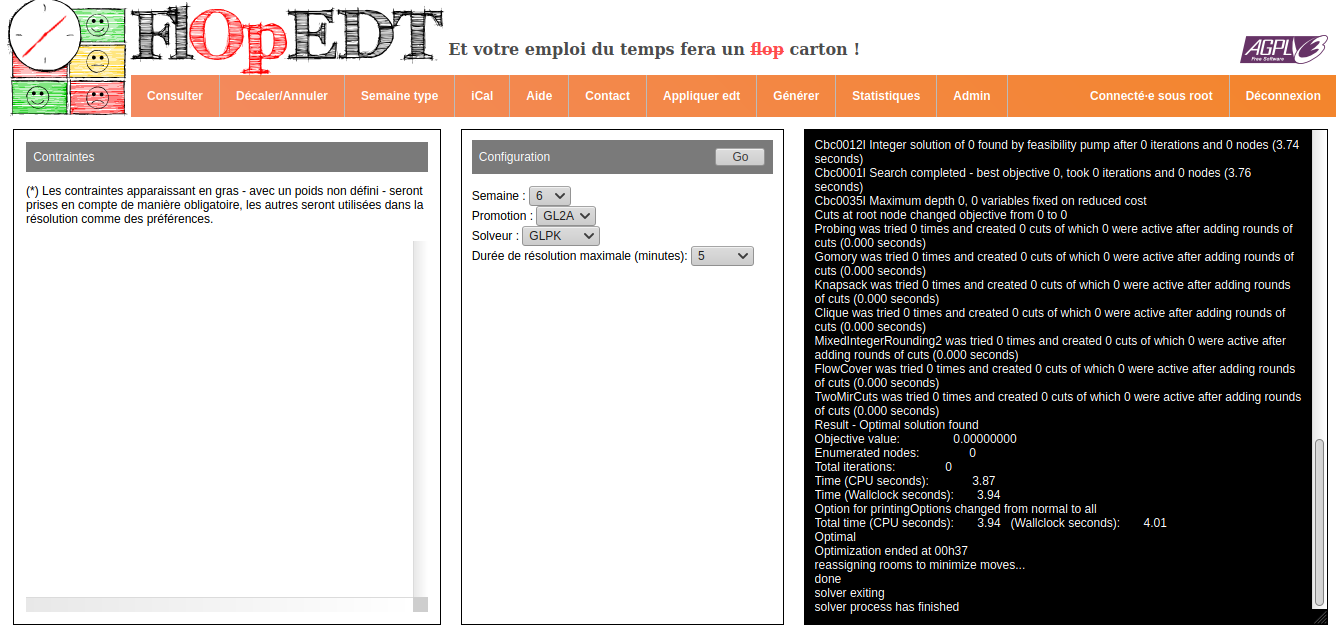
\includegraphics[width=15cm,height=12cm]{img/4.png}
        \caption{Interface générer emploi du temps}
\end{figure}
\newpage

\subsection*{Emploi générée}
Voilà notre emploi du temps, ce dernier peut étre modifié que par le chef de fillière via l'option modifier.
\begin{figure}[H]
      \centering
        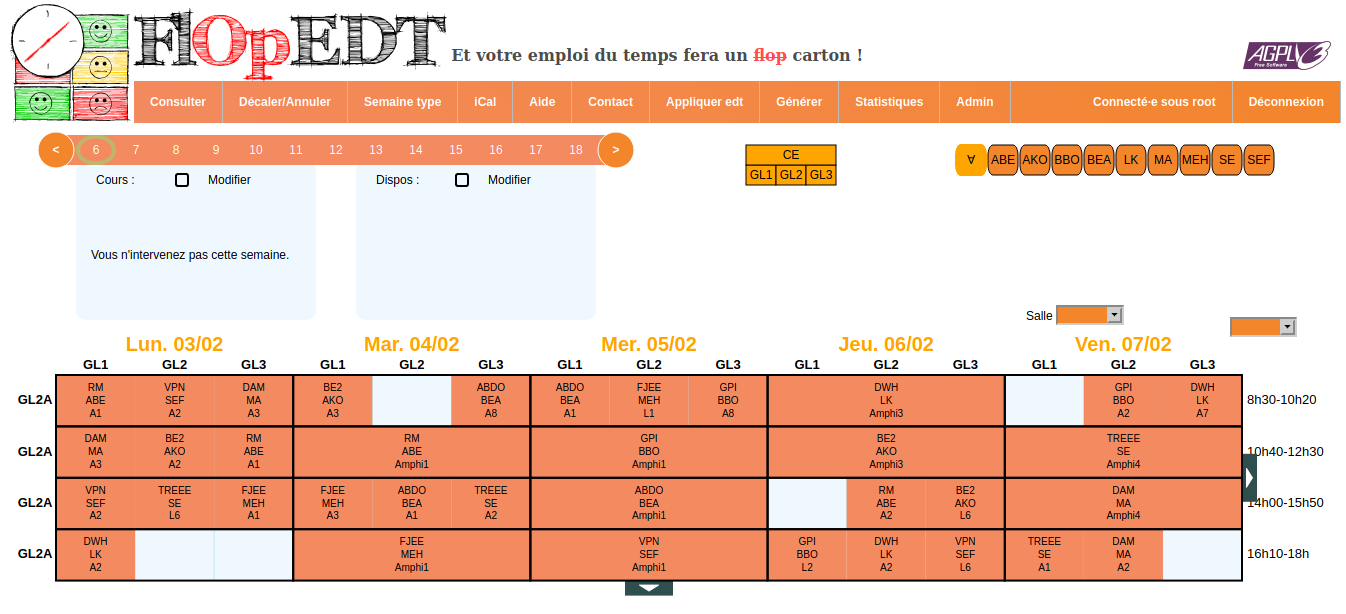
\includegraphics[width=15cm,height=12cm]{img/5.png}
        \caption{Interface Emploi généré}
\end{figure}
\newpage
\subsection*{Sauvegarder emploi du temps}
Si le chef de fillière est satisfait du résultat qu'il a eu, il peut sauvegarder l'emploi du temps pour toute la période.
\begin{figure}[H]
      \centering
        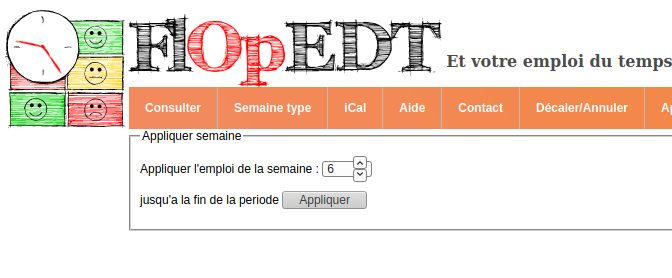
\includegraphics[width=15cm,height=12cm]{img/6.png}
        \caption{Sauvegarder emploi du temps}
\end{figure}
\newpage

\subsection*{Repporter ou annuler un cours}
Si le prof pour une raison quelconque veut repporter ou même annuler un cours, il peut le faire via cette interface, il doit d'abord préciser quel cours et avec quel groupe, et quand il va étre rattrappé.
\begin{figure}[H]
      \centering
        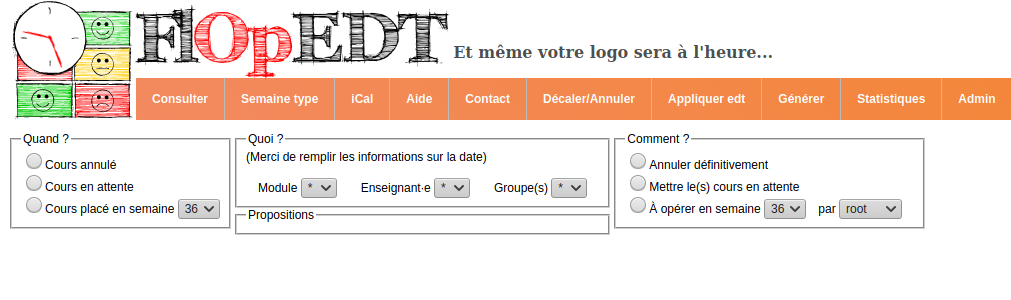
\includegraphics[width=15cm,height=12cm]{img/7.png}
        \caption{Interface repporter et annuler un cours}
\end{figure}
\newpage











\clearpage
\chapter*{Conclusion générale}
Notre projet consiste à améliorer et adapter une application web qui génére l'emplois du temps de Génie Logiciel à l'ENSIAS.


Pour atteindre cet objectif, nous avons commencé par l'analyse de besoin pour délimiter les fonctionnalités à implémenter. Nous avons ensuite abordé l'étude des outils au développement ainsi que la démarche qu'il faut respecter pour réaliser notre projet. Après, nous avons défini la conception de notre système en présentant l'architecture technique de l'application. Finalement, nous avons attaqué la partie réalisation qui consiste à implémenter les fonctionnalités ciblées.


Ce projet de est une expérience très enrichissante. En effet, ce fût une occasion pour nous de mettre en pratique et d'élargir nos connaissances acquises à l'ENSIAS. Il nous a également donné l'opportunité d'intégrer une équipe performante
et de bien connaître son métier. La réalisation du projet nous a aussi permis de raffiner nos capacités de conception et de renforcer nos compétences.


% \input{}
% \cleardoublepage
% \input{}
% \cleardoublepage
% ...

% Appendix______________________________________________________________________



% Bibliography__________________________________________________________________
% Literature (Additional references can be added to the .bib-file manually, or by using, for example, the free application JabRef). Compile in the following order: latex -bibtex -latex -latex
\nocite{*}
\bibliographystyle{ieeetr}
\bibliography{bibliography}
\restoregeometry


\end{document}
